Anhand des Conv\_MaxPool-Netzwerks (CMP) werden sämtliche allgemeinen Ergebnisse und Besonderheiten erläutert. Dabei handelt es sich um ein Deep 
Cascade Klassifikationsnetzwerk, welches in iterativer Weise aufgebaut ist. Das Netzwerk ist ein Convolutional Neural Network mit Padding, 
sodass die räumlichen Dimensionen innerhalb der Convolutional Layer erhalten bleiben. Als Aktivierungsfunktion wird die ReLU-Funktion 
eingesetzt.

\begin{figure}[htpb]
    \centering
    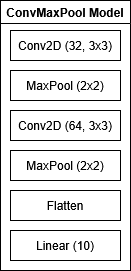
\includegraphics[height=5cm]{../../Graphiken/convmaxpool.png}
    \caption{\label{fig:convmaxpool} 
    \small{Dem CMP-Netzwerk liegen die Layer in exakt der hier von oben nach unten dargestellten Reihenfolge zugrunde.}}
\end{figure}

Alle Layer des ConvMaxPool-Netzwerks sind in Abbildung \ref{fig:convmaxpool} in der korrekten Reihenfolge dargestellt. Dabei gibt die erste 
Zahl eines Convolutional Layers die Anzahl der verwendeten Filter an, während das anschließende Tupel die Größe der Filterkerne spezifiziert. 
Analog wird die Kerngröße auch bei den MaxPooling-Layern angegeben. Das Flatten- sowie das Linear-Layer bilden den Output-Block. Das 
Linear-Layer verfügt über zehn Neuronen, entsprechend der Anzahl der Klassen im Klassifikationsproblem. Jedes Hidden Layer wird über zehn 
Trainings-Epochen optimiert. Ein Early-Stopping-Verfahren kommt nicht zum Einsatz, und für alle Versuchsreihen wird derselbe Zufallsseed 
verwendet.
